La \textit{Management Information Base} (MIB) constituye el modelo de información utilizado por SNMP para representar los recursos administrables de un dispositivo. Aunque su nombre podría sugerir una base de datos convencional, la MIB no corresponde necesariamente a una estructura física almacenada en disco. En realidad, se trata de una representación lógica y estandarizada de los objetos que pueden ser consultados o modificados mediante el protocolo SNMP.

La función principal de la MIB es proporcionar un lenguaje común entre gestores y agentes. Gracias a esta abstracción, una aplicación de gestión puede interpretar la información expuesta por dispositivos de distintos fabricantes sin necesidad de conocer los detalles internos de implementación de cada uno de ellos.

\subsection{Estructura Jerárquica y Object Identifiers (OID)}

La información contenida en una MIB se organiza mediante una estructura jerárquica en forma de árbol. Cada nodo representa un objeto administrable y se identifica de manera única mediante un \textit{Object Identifier} (OID).

Un OID puede entenderse como la ruta completa desde la raíz del árbol hasta un objeto específico. Esta representación garantiza que cada elemento gestionado posea un identificador único a nivel global.

La jerarquía comienza en la raíz del árbol y continúa a través de distintas ramas estandarizadas. La mayoría de los objetos utilizados en la gestión de redes residen bajo el prefijo:

\begin{center}
\texttt{1.3.6.1.2.1}
\end{center}

correspondiente al nodo \textit{mib-2}, definido por los estándares de Internet.

Por ejemplo, el objeto \textit{sysDescr}, utilizado para obtener una descripción textual del dispositivo, posee el siguiente identificador:

\begin{center}
\texttt{1.3.6.1.2.1.1.1.0}
\end{center}

Mientras que los administradores suelen trabajar con nombres simbólicos como \textit{sysDescr}, los mensajes SNMP intercambian internamente los identificadores numéricos correspondientes.

\begin{figure}[H]
\centering
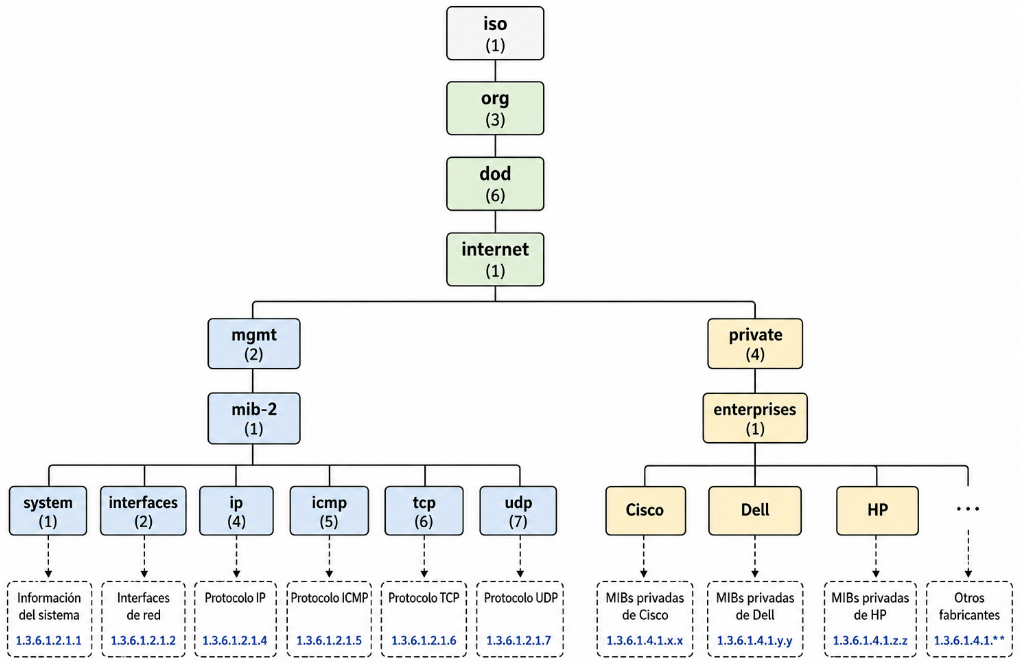
\includegraphics[width=0.85\textwidth]{img/snmp4.png}
\caption{Estructura jerárquica simplificada del árbol OID utilizado por SNMP.}
\label{fig:mib_oid_tree}
\end{figure}

\subsection{Structure of Management Information (SMI)}

La organización y descripción de los objetos de una MIB se encuentra regulada por la \textit{Structure of Management Information} (SMI). Este conjunto de especificaciones define las reglas necesarias para nombrar objetos, describir sus atributos y establecer los tipos de datos permitidos.

La SMI utiliza el lenguaje formal ASN.1 (\textit{Abstract Syntax Notation One}), ampliamente utilizado en protocolos de comunicación para garantizar representaciones precisas y libres de ambigüedades.

Las principales versiones empleadas en SNMP son SMIv1 y SMIv2. Mientras que SMIv1 estableció la estructura básica utilizada por SNMPv1, SMIv2 amplió las capacidades del modelo incorporando nuevos tipos de datos y mecanismos de definición más flexibles.

Entre los tipos de datos más utilizados se encuentran:

\begin{itemize}
\item \textbf{INTEGER}: valores enteros.
\item \textbf{OCTET STRING}: cadenas de caracteres o secuencias de bytes.
\item \textbf{Counter32}: contadores que aumentan monotonamente.
\item \textbf{Gauge32}: valores que pueden aumentar o disminuir.
\item \textbf{TimeTicks}: intervalos de tiempo expresados en centésimas de segundo.
\end{itemize}

La utilización de SMI permite que los objetos definidos por distintos fabricantes mantengan una estructura consistente e interoperable.

\subsection{MIBs Estándar para la Gestión de Servidores}

A medida que SNMP evolucionó, se desarrollaron múltiples módulos MIB especializados para representar distintos aspectos de la infraestructura de red y de los sistemas informáticos.

\subsubsection{MIB-II}

Definida originalmente en el RFC 1213, MIB-II constituye la base de la administración de redes TCP/IP. Organiza la información en grupos funcionales tales como: \textit{system},
\textit{interfaces}, \textit{ip}, \textit{icmp}, \textit{tcp}, \textit{udp}


Estos grupos permiten obtener información general del dispositivo, estadísticas de interfaces de red y métricas asociadas a los principales protocolos de comunicación.

\subsubsection{IF-MIB}

La IF-MIB complementa la información de MIB-II proporcionando estadísticas detalladas sobre las interfaces de red.

Entre los parámetros habitualmente monitorizados se encuentran:

\begin{itemize}
\item Octetos transmitidos y recibidos.
\item Paquetes descartados.
\item Errores de transmisión.
\item Estado operativo de las interfaces.
\item Velocidad configurada de los enlaces.
\end{itemize}

Estas métricas son ampliamente utilizadas para el análisis de rendimiento y la detección de problemas de conectividad.

\subsubsection{HOST-RESOURCES-MIB}

La HOST-RESOURCES-MIB extiende la capacidad de monitorización hacia los recursos internos de servidores y estaciones de trabajo.

A través de este módulo es posible obtener información relacionada con:

\begin{itemize}
\item Uso de CPU.
\item Memoria disponible y utilizada.
\item Sistemas de archivos.
\item Capacidad de almacenamiento.
\item Procesos en ejecución.
\item Tiempo de actividad del sistema (\textit{sysUpTime}).
\end{itemize}

Debido a que estos indicadores reflejan directamente el estado operativo de los servidores, la HOST-RESOURCES-MIB constituye uno de los componentes más importantes para la monitorización de clusters y centros de datos.

\subsection{MIBs Propietarias de Fabricantes}

Además de los módulos estandarizados, SNMP reserva una rama específica del árbol OID para extensiones desarrolladas por los fabricantes.

Estas extensiones se encuentran bajo la rama:

\begin{center}
\texttt{1.3.6.1.4.1}
\end{center}

correspondiente al nodo \textit{enterprises}.

Cada fabricante dispone de un subárbol propio donde puede definir objetos específicos asociados a funcionalidades particulares de su hardware.

Esta capacidad permite exponer información que no forma parte de los estándares generales, incluyendo sensores internos, controladoras de almacenamiento, sistemas de alimentación redundante y plataformas avanzadas de administración remota.

Algunos ejemplos ampliamente utilizados son:

\begin{itemize}
\item Dell iDRAC.
\item HP iLO.
\item Cisco UCS.
\end{itemize}

Mediante estas extensiones es posible monitorizar parámetros como temperatura del chasis, estado de ventiladores, fallos de discos, fuentes de alimentación redundantes y alertas de hardware específicas de cada fabricante.

En conjunto, los OID proporcionan el mecanismo de direccionamiento, la SMI define el modelo de representación y las distintas MIBs especifican los objetos concretos que pueden ser gestionados. Esta combinación constituye la base sobre la cual los sistemas SNMP realizan la supervisión y administración de infraestructuras de red y servidores.
